\section{Polovodičové paměti}
Paměť je médium, které umožňuje uchovávat informace.
Základní paměťová buňka uchovává jeden bit informace - buďto logickou 0 nebo logickou 1.
Osm takových buňek tvoří jeden bajt.
Paměťové prvky jsou spojeny řádkovými a sloupcovými vodiči, pomocí kterých je možné je elektronicky ovládat.\\ \\
Parametry pamětí:
\begin{description}
    \item [Kapacita {[B]} -] Množství informací, které lze do paměti uložit
    \item [Přístupová doba {[s]} -] Doba, od zadání požadavku, než paměť zpřístupní požadovanou informaci
    \item [Přenovová rychlosti {[B/s]} -] Množství dat, které lze přečíst/zapsat za sekundu
    \item [Šířka toku dat {[b]} -] Počet bitů, které se po sběrnici přenášejí současně
    \item [Cena za bit {[Kč/b]} -] Cena za jeden bit paměti.
    \item [Spolehlivost {[s]} -] Střední doba mezi 2 poruchami
\end{description}
\subsection{Základní rozdělení}
\subsubsection{ROM - Read Only Memory}
\begin{multicols}{2}
    Z paměti lze pouze číst.
    Obsah paměti se po vypnutí napětí neztrácí.
    Vyrábí se pomocí speciální metalické masky.
    Jsou drahé.
    Mohou být realizované jako dvojice spojených a nespojených vodičů.

    Dále mohou být realizované pomocí tranzistorů buďto TTL nebo MOS.
    Paměti realizované tímto způsobem jsou připojené na adresný vodič, což znamená logickou 0 na výstpupu, či naopak.
    \columnbreak

    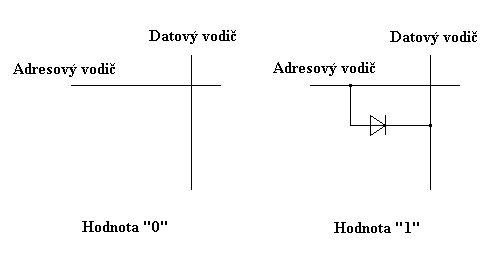
\includegraphics[width=\linewidth]{TVY-POS/Polovodicove-pameti/ROM.png}
\end{multicols}
\begin{multicols}{2}
    \begin{center}
        TTL \\
        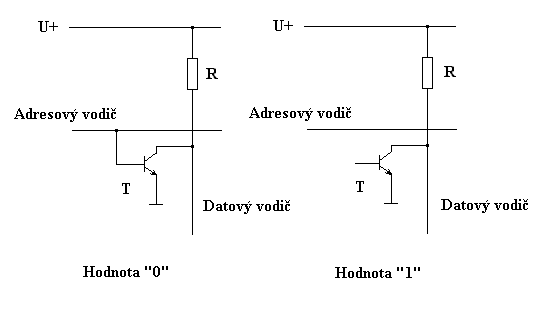
\includegraphics[width=1.2\linewidth]{TVY-POS/Polovodicove-pameti/ROMTTL.png}
    \end{center}
    \columnbreak
    \begin{center}
        MOS \\
        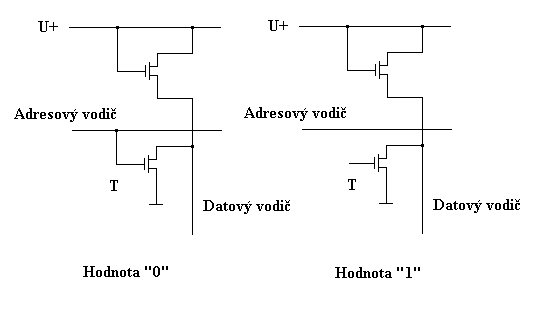
\includegraphics[width=1.2\linewidth]{TVY-POS/Polovodicove-pameti/ROMMOS.png}
    \end{center}
\end{multicols}
\subsubsection{RWM - Read Write Memory}
Je možné zapisovat do a poté číst z této paměti.
Realizované pomocí níže uvedených technologií.
\newpage
\subsubsection{PROM - Programable Read Only Memory}
\begin{multicols}{2}
    Od výroby neobsahuje pevnou informaci, po zápisu první informace už nejde zapisovat znova a paměť funuje stejně jako ROM.
    Vyrobena je s hodnotou samých logických 1.\\
    Zápis informace se provádí vyšší hodnotou elektrického proudu (cca 10 mA), která způsobí přepálení tavné pojistky a tím i definitivně zápis hodnoty 0 do příslušné paměťové buňky.\\
    Vyrábí se podobně jako paměti ROM, akorát se všechny spoje vyrobí jako spojené pomocí pojistky z Niklu a Chromu (NiCr)\\
    \columnbreak

    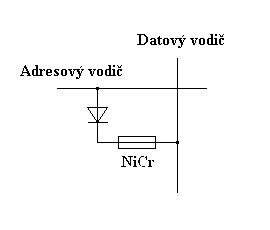
\includegraphics[width=0.7\linewidth]{TVY-POS/Polovodicove-pameti/PROM.png}
\end{multicols}
Existují i paměti PROM realizované pomocí bipolárních multiemitorových tranzistorů, které fungují na opačné logice.
\begin{multicols}{2}
    \subsubsection{EPROM - Erasable Programable Read Only Memory}
    Paměť EPROM je statická a energeticky nezávislá pamět.
    Zapisuje se do ní pomocí speciálního porogramátoru a zápis trvá 10 až 20 minut.
    Paměť se maže pomocí působení ultrafialového záření po dobu asi 30 minut.
    Paměť funguje na speciálních unipolárních tranzistorech, který udrží náboj na jejich přechou několik let.
    Vzhled paměti je charakteristická malým okénkém v pouzdře švábu, ve kterém byl paměťový čip.
    Okénko se při práci zakrývalo, aby nedocházelo ke ztrátě inforamcí.
    \columnbreak
    \subsubsection{EEPROM - Electrically Erasable Programable Read Only Memory}
    Chová se podobně jako EPROM, ale data je možné smazat elektricky.
    Programování je tudíž možné přímo v systému a naprogramování trvá méně než minutu.
    Pro výrobu se využívají speciální tranzistory s vrstvou nitridu křemíku a oxidu křemičitého mezi kterým je uchován el. náboj, který se vkládá na jejich přechod.\\
\end{multicols}

\subsubsection{RWM-RAM - Read Write Memory-Random Access Memory}
Energeticky závislé paměti rychlejší než ROM a mají větší kapacitu.
Jsou určené k přímé spolupráci s procesorem.
Dělí se na dynamické a statické
\subsubsection{SRAM}
\begin{multicols}{2}
    Uchovávají informaci, dokud jsou připojené k el. napájení.
    Paměťová bunka je realizována jako bistabilní klopný obvod.
    U těchto pamětí se používají dva datové vodiče - DATA a \textoverline{DATA}, hodnota na tomto vodiči je vždy opačná než hodnota uložená v paměti, proto je nutné ji negovat.
    Jeden pro čtení a druhý pro zápis.
    Mezi výhody patří nížká přístupová doba (~10ns).
    Nevýhodou je složitost a vyšší výrobní náklady.
    V dnešní době se používají pro paměti typu cache.
    \columnbreak

    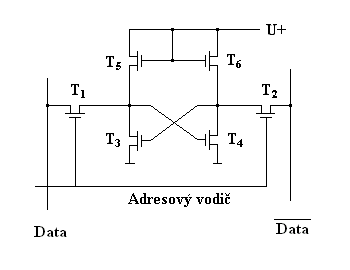
\includegraphics[width=0.8\linewidth]{TVY-POS/Polovodicove-pameti/SRAMM.png}
\end{multicols}
Při zápisu na adresový vodič se umístí hodnota log. 1, na DATA se přivede zapisovaná hodnota a podle hodnoty se otevřou a zavřou určité tranzistory.
Při čtení se opět na adresný vodič přivede log. 1 a podle stavů tranzisorů se na vodiči \textoverline{DATA} obdrží opačná hodnota buňky.
\subsubsection{DRAM}
Informace je uložena pomocí el. náboje na kondenzátoru.
Náboj má tendenci se vybíjet i když je pamět připojena k el. napájení, proto se musí provádět \textbf{refresh}.
\begin{multicols}{2}
    Při zápisu se na adresný vodič přivede hodnota log. 1.
    Na datový vodič se přijede zapisovaná hodnota, která buďto vybije nebo nabije kondenzátor.
    Čtení probíbá desktruktivně, což znamená že se po čtení musí informace opět zapsat.
    Po přivedení log. 1 na adresný vodič se podle stavu buďto vybije náboj v kondenzátoru, kterého náboj se převede na Datový vodič a nebo ne.\\
    \columnbreak

    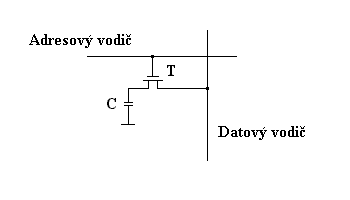
\includegraphics[width=0.8\linewidth]{TVY-POS/Polovodicove-pameti/DRAM.png}
\end{multicols}
Mezi výhody patří jednoduchost a nízké výrobní náklady, zároveň pamět dovoluje vysokou integraci.
V dnešní době se používají pro operační paměti.
Nevýhodou je vyšší přístupová doba (~70ns) a nutnost provádět refresh.
Existují různé druhy DRAM:
\begin{description}
    \item[SDRAM]- používali se dříve, pracují na stejném taktu jako sběrnice
    \item[DDR]- přenášejí data na obou hranách hodin
    \item[DDR2]- pracují s polovniční vnitří frekvenci
    \item[RDRAM]- používá menší sběrnici, měla umožnit využití větší počet kanálů
    \item[CMOS-RAM]- mají malou spotřebu, zapisují se do nich parametry BIOSu. Po vypnutí PC se napájí pomocí baterie Li-ion většinou z obvodu hodin reálného času na MB.
\end{description}
\subsubsection{FLASH}
Obdoba EEPROM paměti.
Jsou to paměti statické a elektricky nezávislé.
Programují se také přímo v počítači.
Paměti není nutné z počítače pro programování vyjmout.
Zapisuje so do ní po blocích a celá pamět se zapíše v rámci sekund.
Pracuje se s nimi jako s pamětmi RAM, ale po odpojení se jejich obsah nesmaže.
Při použití k uložení BIOSu, tak se BIOS dá aktualizovat.
\subsection{R/W cyklus buňky}
\begin{multicols}{2}
    Vždy je udána adresa paměťového místa, se kterým se pracuje.
    Adresa je přivedena na vstup dekoréru, která podle adresy nastaví adresový vodič na logickou 1.
    Jestliže buňkou na tomto adresném vodiči projde logická 1 na datový vodič, tak je hodnota bitu logická 1.
    V případě že buňkou logická 1 neprojde, pak je hodnota bitu 0.
    U zápisu je dána opět adresa místa, kam se bude zapisovat, poté se nastaví hodnoty jednotlivých bitů a zapíšou se.\\
    \columnbreak

    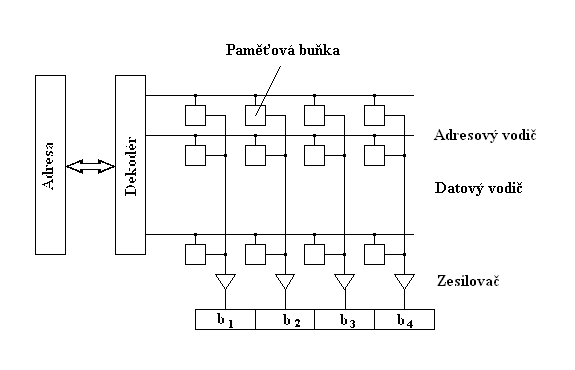
\includegraphics[width=0.9\linewidth]{TVY-POS/Polovodicove-pameti/memorystructure.png}
\end{multicols}
